
%(BEGIN_QUESTION)
% Copyright 2010, Tony R. Kuphaldt, released under the Creative Commons Attribution License (v 1.0)
% This means you may do almost anything with this work of mine, so long as you give me proper credit

Tegn inn koblingene som er nødvendige for å koble en nærhetsbryter til inngangkanal \texttt{Ix.8} på en Siemens SM 321 DI modul (model 6ES7321-1BP00-0AA0). Internt koblingskjema for en inngang (\texttt{Ix.0} vises som en referanse for alle innganger. 


$$\includegraphics[width=15.5cm]{i04544x01.eps}$$

Finn ut om dette er en \textit{sinking} eller en \textit{sourcing} nærhetsbryter og strømretning for alle tilkoblinger til modulen. 


\vfil 

\underbar{file i04544}
\eject
%(END_QUESTION)





%(BEGIN_ANSWER)

This particular proximity switch {\it sinks} current from the input module (arrows drawn in the direction of conventional flow):

$$\includegraphics[width=15.5cm]{i04544x02.eps}$$

Note that the PLC input card has the ability to either source or sink current at each input, owing to the full-wave bridge rectifier which guarantees the optocoupler's LED will receive current in the correct direction no matter how current may enter or exit the input terminal.

%(END_ANSWER)





%(BEGIN_NOTES)


%INDEX% PLC, I/O: discrete I/O device wiring

%(END_NOTES)


